\chapter{Reinforcement Learning}\label{chapter:architecture}
In this chapter we explain the some concepts of Reinforcement Learning, a starting technique of RL and the three techniques that we used in this work. It is dived in 5 sections: explanation of the concepts and definitions of Reinforcement Learning, Q-Learning, Deep Q Network, Dueling Double Deep Q Networks and Deep Deterministic Policy Gradient.

\section{Concepts and Definitions}
Reinforcement Learning is a field of machine learning that studies a computational way to learn how to reach an objective taking actions over the time to maximize a reward function depending on environment's reaction of each action taken. To understand the RL techniques that we explain, we must learn some concepts and definitions. 

An \textbf{agent} is the actor that will interact with the environment and understand if the action that it took was good or bad for the task. The \textbf{environment} is everything that the agent will interact, eg.: if we are drinking water the environment is the kitchen, the  bottle of water, how much water last in the bottle. The environment is formally announced as a a Markov Decision Process (MDP), \cite{mdp}. A MDP is a 4-tuple ($S, A, P_a, R_a$) where:
\begin{itemize}
    \item S is a finite set of state that describe the features of the environment. A state $s$ describes the environment in a certain time $t$.
    \item A is a finite set of actions that the agent can take at any time. An action $a$ describes an action taken in a state $s$.
    \item $P_a(S,S') = Pr(s_{t+1}=s' | s_t=s, a_t=a)$ is the probability of agent taking the action $a$ on state $s$ at time $t$ will lead to state $s'$.
    \item $R_a(S,S')$ is the reward for the agent taking an action $a$ on a state $s$ at time $t$ leading on a state $s'$.
\end{itemize}

\begin{figure}[H]
    \centering
    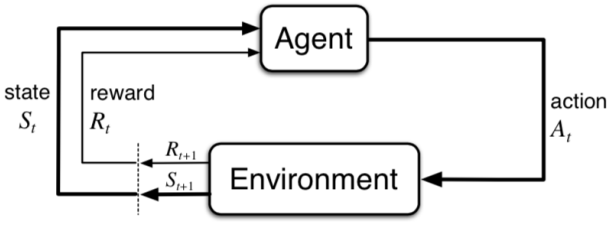
\includegraphics[scale=0.5]{images/rl.png}
    \caption{Example of model of Reinforcement Learning. Image from \cite{rlsutton}.}
    \label{fig:my_label}
\end{figure}

Some definitions of RL:

\begin{defn}A \textbf{Policy} $\pi$ is a rule to select actions. It can be deterministic, if the state maps the actions, or stochastic,  when the action choice depends on a probability distribution. The optimal policy is called $\pi^*$. \end{defn}

\begin{defn}An \textbf{Episode} is analogous to an epoch in RL. An Episode $\tau$ is a sequence of 3-tuple ($s, a, r$). \end{defn}

\begin{defn}A \textbf{Step} is the acting of the agent. Each episode have certain number of steps. In our domain, the agent can take approximately 300 steps until the current episode finishes.\end{defn}

\begin{defn}The \textbf{Experience Replay} buffer (or \textbf{Memory}) of an agent is analogous to a dataset in RL. It is the previous $N$ episodes passed, with $N$ being defined by the programmer.\end{defn}

\begin{defn}The \textbf{Value} of a state $V(s)$ describes the expected return after state $s$. It can be interpreted as how good $s$ can be, based on previous memories.\end{defn}

\begin{defn}The \textbf{Q-Value} $Q(s, a)$ describes how good is to take an action $a$ in a given state $s$. The optimal \textit{Q-Value} is called $Q^*$. The \textit{Q-Value} is formally described as:
    \begin{figure}[H]
        \centering
        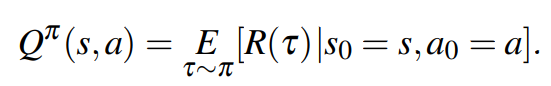
\includegraphics[scale=0.35]{images/qvalue.png}
        \caption{Formal description of \textit{Q-Value}. Image from \cite{tgze}.}
        \label{fig:qvalue}
    \end{figure}
\end{defn}

\begin{defn}The \textbf{Bellman Equation} is the base of Reinforcement Learning. It can describe $V(s)$ and $Q(s,a)$ recursively based on the actual 4-tuple $(s, a, r, s')$ and t-tuple $(s, a, r, s', a')$ respectively. See Equations \ref{eq:value}, \ref{eq:qvalue} and \ref{eq:reward}.$\gamma$ is the discount rate which represents how much $Q(s', a')$ can impacts on $Q(s,a)$.

\begin{equation}
    V(s) = \max_a(R + \gamma V(s'))
    \label{eq:value}
\end{equation}

\begin{equation}
    Q(s,a) = \max_a(R + \gamma Q(s', a'))
    \label{eq:qvalue}
\end{equation}

\begin{equation}
    R = R(s, a, s')
    \label{eq:reward}
\end{equation}

 \end{defn}

\section{Q-Learning}\label{section:qlearning}
Q-Learning (\cite{qlearning}) is one of the basics algorithms of Reinforcement Learning. It works based on a matrix called \textit{Q-Table} where the columns represents the actions that the agent can take and the rows represents the set $S$ of states. The \textit{Q-Table} is updated for each step based on the Equation \ref{eq:qfunction} which is called \textit{Q-Function}, an adaption of the Bellman's Equation. See Figure \ref{fig:qtable}. The algorithm does the work when the environment has a small discretized state space, otherwise it would take a very long time to the matrix converge. Other problem of the technique is the keeping of a local maximum due to the lack of generalisation of states.
\begin{equation}
\underbrace{\text Q(s,a)}_{\scriptstyle\text{Q-Value}}=Q(s,a)+\mkern-34mu\underset{\text{Learning rate}}{\underset{\Bigl|}{\alpha}}\mkern-30mu[\underbrace{R(s,a)}_{\scriptstyle\text{Reward}}+\mkern-30mu\underset{\text{Discount rate}}{\underset{\Biggl|}{\gamma}}\mkern-75mu\overbrace{\max Q'(s',a')}^{\scriptstyle\substack{\text{Maximum predicted reward, given} \\ \text{new state and all possible actions}}}\mkern-45mu-Q(s,a)]
\label{eq:qfunction}
\end{equation}

\begin{figure}[H]
    \centering
    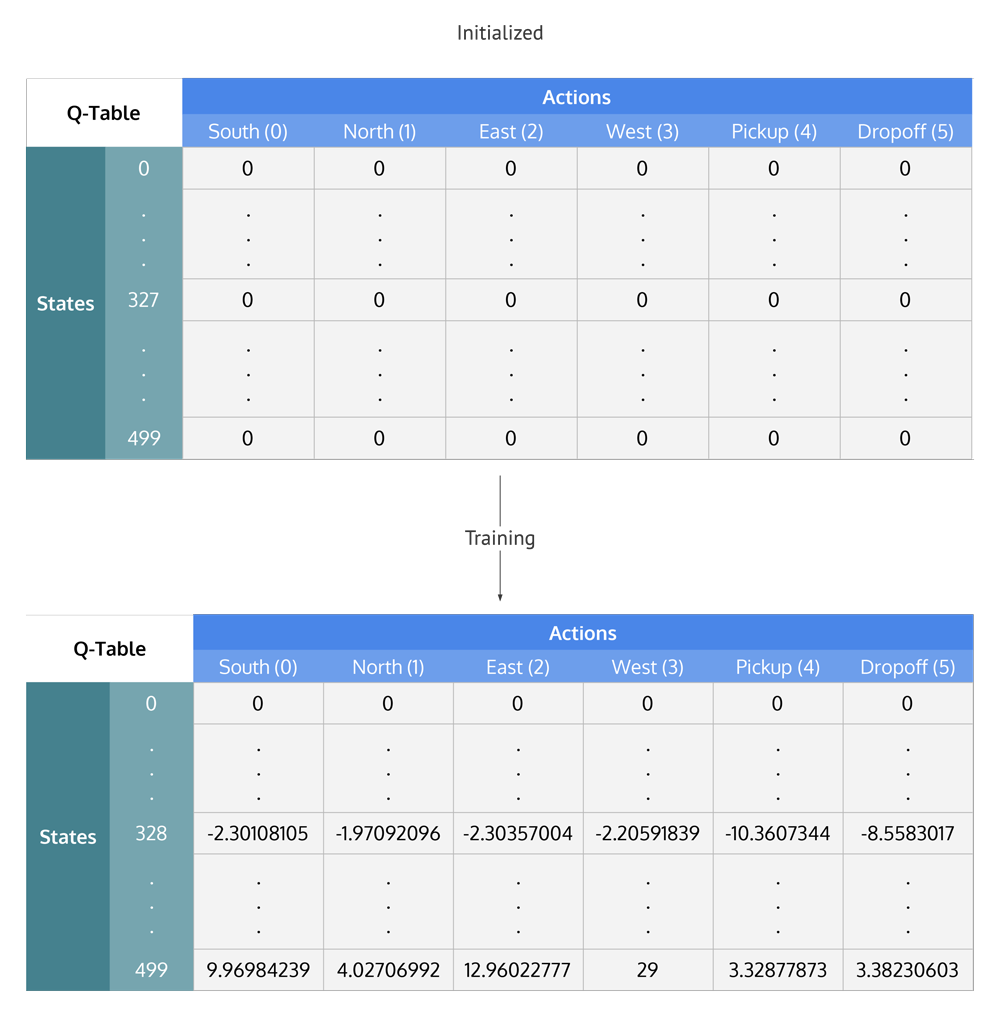
\includegraphics[scale=0.35]{images/Q-Learning_Matrix_Initialized_and_After_Training.png}
    \caption{Example of Q-Table. By LearnDataSci - Own work - Article, CC BY-SA 4.0, https://commons.wikimedia.org/w/index.php?curid=69947708, accessed on 15/09/2019.}
    \label{fig:qtable}
\end{figure}

\section{Deep Q Network}\label{section:dqn}
Deep Q Network (DQN) is the Deep Learning approach for Q-Learning created by \cite{dqn}. Although basic (comparing with today's techniques), it opened the eyes for Reinforcement Learning achieving impressive results with Atari's games. DQN solves the problems of Q-Learning using a non-linear function (Neural Networks) as a $Q*$ approximator. The loss function of the DQN changes every iteration $i$ and is derived from the Bellman's Equation. See Figure \ref{fig:dqnfuncloss}. $\theta$ represents the network's weights and $\rho(s,a)$ is the probability distribution over states and actions, also called behaviour distribution. DQN's algorithm is in the Figure \ref{fig:dqn_alg}.

\begin{figure}[H]
    \centering
    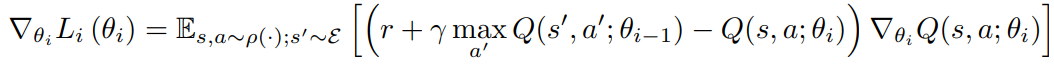
\includegraphics[scale=0.3]{images/dqn_lossfunc.png}
    \caption{$L_i(\theta_i)$ as loss function of DQN's Neural Networks.}
    \label{fig:dqnfuncloss}
\end{figure}

\begin{figure}[H]
    \centering
    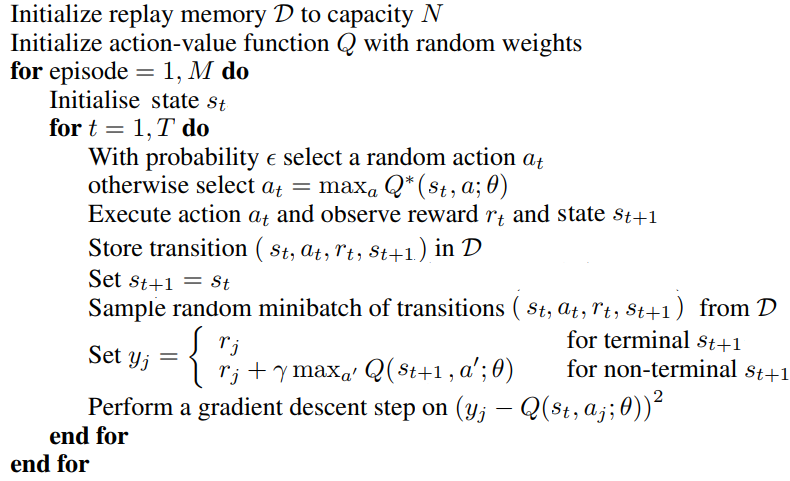
\includegraphics[scale=0.5]{images/dqn_alg.png}
    \caption{Deep Q Networks algorithm with Experience Replay.}
    \label{fig:dqn_alg}
\end{figure}

\section{Double Deep Q Networks}\label{section:ddqn}
Deep Q Networks brings a maximization bias learning due to the $max_a' Q^*(s',a')$ part of the Q-Learning equation. In other words, it says that some Q-Values are more valuables than it should. And such overestimation can be problematic. \cite{doubledqn} brought the idea of Double Deep Q Networks to cure the overestimation problem based on the cure for the same problem in Q-Learning with Double Q-Learning, \cite{doubleqlearning}.

\cite{doubledqn} proposes a solution involving two $Q*$ estimators, one to update the other with certain rate of averaging $\tau$. Using it, the \textit{Q-Value} will be unbiased by the opposite estimator of the action selector. The algorithm proposed is in Figure \ref{fig:doubledqn_alg}. See Figure \ref{fig:doubledqnoverestim} for the results.

\begin{figure}[H]
    \centering
    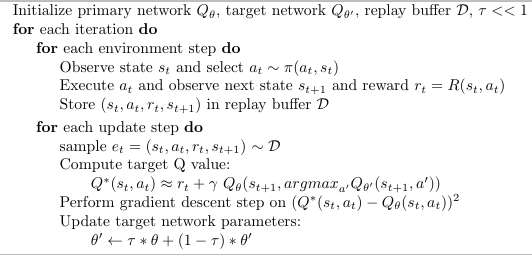
\includegraphics[scale=0.8]{images/doubledqn_alg.png}
    \caption{Double DQN algorithm. Image from https://towardsdatascience.com/double-deep-q-networks-905dd8325412, accessed on 15/11/2019.}
    \label{fig:doubledqn_alg}
\end{figure}

\begin{figure}[H]
    \centering
    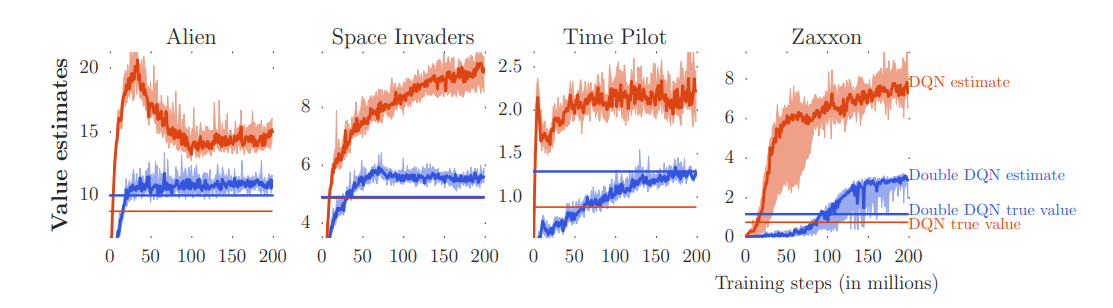
\includegraphics[scale=0.4]{images/double_dqn_estimation.png}
    \caption{Q-Value in fuction of time for some Atari games: estimation and truth values for DQN and Double DQN. Image from \cite{doubledqn}.}
    \label{fig:doubledqnoverestim}
\end{figure}


\section{Dueling Double Deep Q Networks}\label{section:ddqn}
Dueling Double Deep Q Networks (DDQN) brings the idea of Double DQN and a plus. \cite{DDQN} propose a dueling architecture for the final layers of the Neural Networks. It separates explicitly the state values and state-dependent action advantage via two different Neural Networks. 

The motivation of the technique is that some environments do not depend fully of an action, sometimes if the agent does not do some action or does a single action, it takes more reward than taking multiple actions. It applies very well on our multi-agent context, for example if the right winger is intercepting the ball, it's more valuable to the left winger stays on it's position than intercepting.

The new \textit{Q-Function} will be naively described as Equation \ref{eq:ddqn}. Due to identifiability problem of sum, the back propagation can not tell what is $V(s) or A(s,a)$, so \cite{DDQN} propose the Equation \ref{eq:ddqn_best} to train the agent.

\begin{equation}
    Q(s,a;\theta, \alpha, \beta) = V(s; \theta, \beta) + A(s, a; \theta, \alpha)
\label{eq:ddqn}
\end{equation}

\begin{equation}
    Q(s,a;\theta, \alpha, \beta) = V(s; \theta, \beta) + (A(s, a; \theta, \alpha) - \frac{1}{A}\sum_{a'}A(s, a'; \theta, \alpha))
\label{eq:ddqn_best}
\end{equation}

\begin{figure}[H]
    \centering
    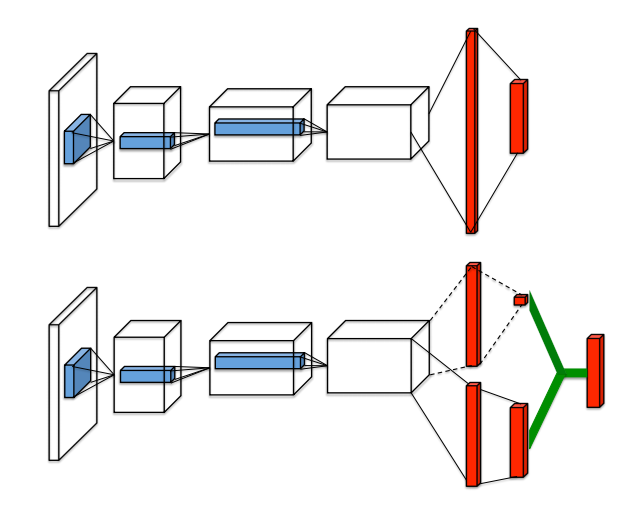
\includegraphics[scale=0.4]{images/dddqn.png}
    \caption{Deep Q Networks architecture against Dueling Deep Q Networks architecture. Image from \cite{DDQN}}
    \label{fig:ddqn}
\end{figure}

\section{Deep Deterministic Policy Gradient}\label{section:ddpg}
There is another branch of RL that studies the Policies and Values themselves. It is like the idea of a DDQN, where there is a Critic and an Actor algorithm, see Figure \ref{fig:acex}. Based on that architecture, \cite{DDPG} develop the Deep Deterministic Policy Gradient (DDPG). The DDPG tries to learn an optimal deterministic policy $\mu^*$.

\begin{figure}[H]
    \centering
    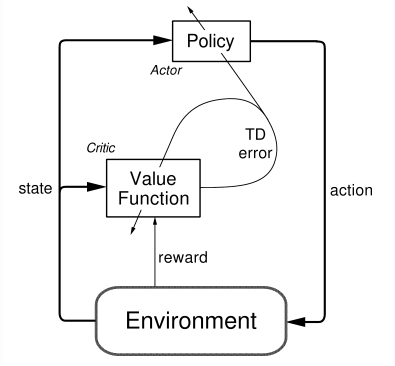
\includegraphics[scale=0.5]{images/AC_example.png}
    \caption{Illustration of an Actor Critic system. Image from \cite{rlsutton}.}
    \label{fig:acex}
\end{figure}

The input of the Actor is the current state and the output is a single real value representing an action chosen from a continuous action space. The output of the Critic is $V(s)$ where $s$ is the current state. See Figure \ref{fig:ddpgalg} to check DDPG's algorithm.


\begin{figure}[H]
    \centering
    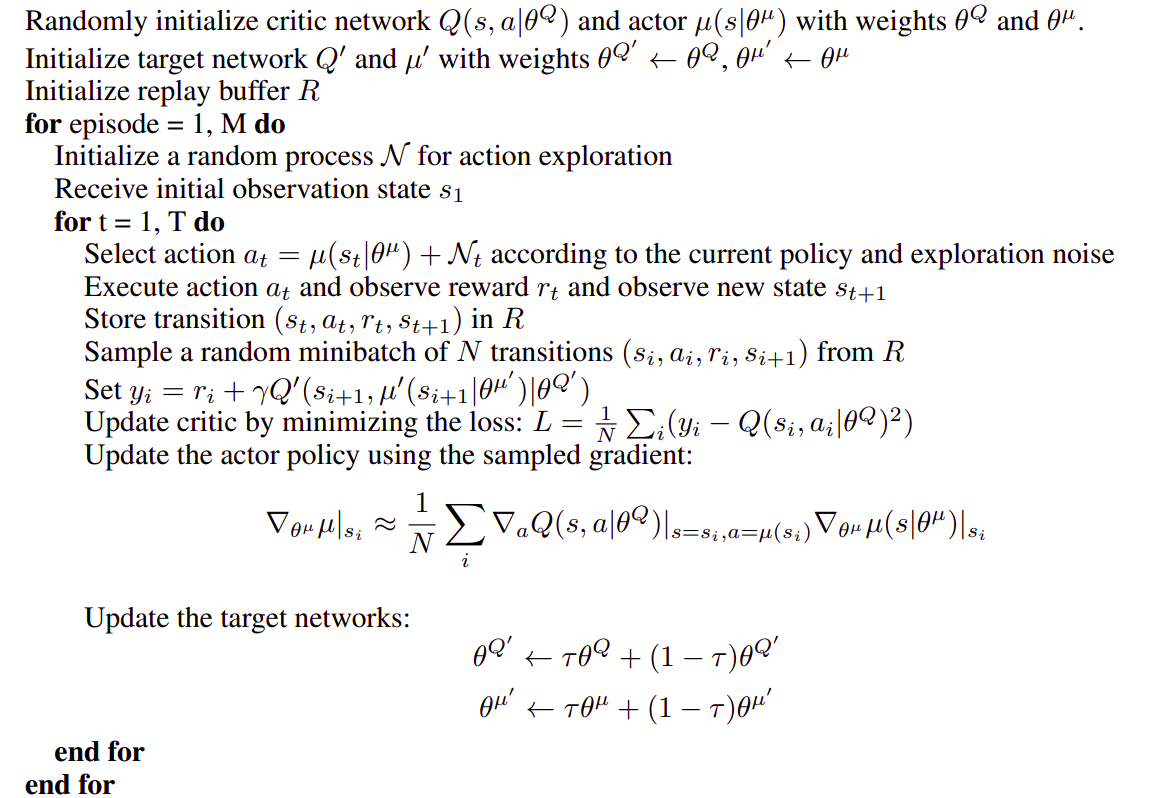
\includegraphics[scale=0.3]{images/ddpgalg.png}
    \caption{Deep Deterministic Policy Gradient algorithm. Image from \cite{DDPG}.}
    \label{fig:ddpgalg}
\end{figure}
